% !TEX root = src/bachelorArbeit/main.tex
\documentclass[german,report]{tudo-raumplanung-thesis-report}

\usepackage{cite}
\usepackage{url}
\usepackage{wrapfig}
\usepackage{needspace}
\usepackage{geometry}
\usepackage{layout}
\geometry{
    left=3cm,
    right=2cm,
    top=2cm,
    bottom=2cm,
    showframe=false
    %textwidth=8cm,  
    %marginpar=3cm
    }

\usepackage{helvet}
\renewcommand{\familydefault}{\sfdefault}

\usepackage[german]{babel}

\usepackage[]{graphicx}

% Provide your title
\title{Entwicklung einer Methodik zur optischen Analyse
spannkraftinduzierter Deformationen additiv gefertigter Bauteile}

% Author name(s)
% organised into two columns if more than 10 authors are provided
\storeauthors\authors{
    {Thieme, Niklas}
}

% Provide the examiners' names.
\storereviewers\reviewers{
    {Jun.-Prof.\ Dr.\ rer.\ nat.\ Great Examiner}
    {Prof.\ Dr.-Ing.\ Fantastic Examiner}
}

\begin{document}
%\centering

\newpage

\tableofcontents

\newpage

% 1_EinleitungMotivation_tex
\chapter{Einleitung}

In den letzten Jahren hat die additive Fertigung (AF), auch bekannt als 3D-Druck, 
zunehmend an Bedeutung in der Industrie gewonnen~\cite{JADHAV20222094}. 
Diese innovative Technologie 
ermöglicht die schichtweise Herstellung komplexer Bauteilgeometrien und bietet im 
Vergleich zu traditionellen Fertigungsverfahren einen höheren Grad an 
Gestaltungsfreiheit. Trotz vieler Vorteile stehen Hersteller vor 
Herausforderungen bezüglich der Oberflächenqualität und Maßhaltigkeit 
der gefertigten Werkstücke~\cite{SCHNECK201919}.
Herausforderungen können die Bauteilgeometrie, die möglichen Materialien oder 
den Herstellungsprozess betreffen.
Die Herausforderungen bei der Bauteilgeometrie umfassen die minimalen 
Wandstärken sowie das maximale Bauteilvolumen, das von den technischen 
Spezifikationen des verwendeten 3D-Druckers abhängt. Für die AF stehen 
verschiedene Materialien zur Verfügung, 
die sich jedoch von den, in der konventionellen, spanenden Fertigung 
verwendeten Werkstoffen unterscheiden. In der AF werden hauptsächlich Legierungen 
auf Basis von Titan, Aluminium, Nickel oder Chrom eingesetzt. Diese Materialien
müssen zudem in einer für das Verfahren geeigneten Form vorliegen, 
meistens in Form von Pulver oder Draht. Der Prozess zur Herstellung von 
Pulver oder Draht aus diesen Materialien ist kostenintensiv und schränkt
die Auswahl der verwendbaren Materialien ein. Aufgrund der 
schichtbasierten Natur der AF sind Stützstrukturen 
notwendig, um Bauteile mit geometrischen Formen, die Überhänge aufweisen, 
erfolgreich produzieren zu können. \label{drawbacks_af}
~\cite{Vranic.2017}

Einige dieser Herausforderungen, können durch Nachbearbeitung des Bauteils 
gelöst werden. Dazu gehört das Entfernen der Stützstrukturen und die Verbesserung
der Oberflächenqualität.
Für den Nachbearbeitungsschritt muss das Bauteil in seiner Position und Lage im Bauraum
der Werkzeugmaschine fixiert werden. Die hierzu aufzubringenden Spannkräfte 
können die filigranen Bauteile elastisch, in Extremfallen auch plastisch, verformen, 
sodass eine maßhaltige spangebende Nachbearbeitung verhindert wird. 
Um den Spannprozess und dessen Auswirkungen auf das Bauteil hinsichtlich 
der erzielbaren geometrischen Genauigkeit optimieren zu
können, ist eine Quantifizierung der spannkraftinduzierten Deformation notwendig.~\cite{newMethod}

Im Rahmen dieser Bachelorarbeit wird deshalb eine Methodik zum Erkennen und 
analysieren einer Deformation entwickelt. Das Ziel dieser Methode ist es, 
mithilfe von optischen Informationen zu additiv gefertigten Bauteilen eine 
Deformation zu erkennen, wie sie zum Beispiel auftreten kann, wenn ein Bauteil 
in einem Schraubstock fixiert wird.

Das Verfahren soll auf verschiedenen Bauteilgeometrien anwendbar sein, daher werden 
möglichst wenig Annahmen über die Bauteilgeometrie getroffen.
Im Verlauf dieser Arbeit werden erst die theoretischen Grundlagen, die für die 
entwickelte Methode notwendig sind dargestellt. 
Anschließend wird das Vorgehen der Methode vorgestellt und die einzelnen 
Schritte erläutert. Das Verfahren besteht aus mehreren Schritten die sich in 
Datenerfassung, Datenaufbereitung, Stitching und Deformationserkennung 
einteilen lassen.

Nach der Vorstellung des Verfahrens wird die Funktion der Methodik anhand eines 
Demonstratorbauteils das in einem Schraubstock fixiert und mit mehrere Kraftstufen 
angezogen wurde, validiert. Hier wird die erkannte Deformation bewertet und 
verschiedene Materialien und Herstellungsverfahren verglichen.

Ziel dieser Arbeit ist es zusätzlich, die entwickelte Methodik in einer einfach
benutzbaren Anwendung umzusetzen. Die Funktionsweise dieser Anwendung wird 
nach der Validierung der Methodik dokumentiert. Außerdem werden verschiedene 
Optimierungen dargelegt, die das Verfahren zeit- und speichereffizienter machen
und die Genauigkeit der Ergebnisse verbessern.

Zum Abschluss dieser Arbeit wird ein Fazit gezogen, in dem die erzielten 
Ergebnisse eingehend diskutiert werden. Zudem wird ein Ausblick auf 
mögliche zukünftige Entwicklungen und weiterführende Forschungsansätze gegeben.





\newpage

\documentclass[../main.tex]{subfiles}
\begin{document}

\section{Stand der Technik}

\subsection{Additive Fertigung}

Additive Fertigung, unabhängig von dem Werkstoff, ist ein Bereich im dem viel
geforscht und innoviert wird. In fast jedem Industriebereich wird versucht ein
bestehendes Design oder Modell zu optimieren und verbessern. \cite{newMethod}
Sei es hinsichtlich Qualität oder Kosteneffizienz. Addtive Fertigung bietet bei 
dieser Optimierung viele Vorteile gegenüber spanenden Fertigungsverfahren, da 
Additive Fertigung einen höheren Grad der Gestaltungsfreiheit bietet. 
Additive Fertigung ist eine Resource die Benutzern ermöglicht komplexe 
Bauteilgeometrien zu erstellen ohne die Limitierung von konventionellen spanenden 
Herstellungsverfahren, wie hoher Materialverschleiß oder die Notwendigkeit von 
spezialisierten Werkzeugen. \cite{Vafadar.2021} 

Außerdem können mit Additiver Fertigung Stückzahlen drastisch reduziert werden.
Werkstücke können bei Bedarf gefertigt werden was die Notwendigkeit für Lagerstätten
größtenteils eliminiert. Zusätzlich können die Teile genau dort herstellt werden wo 
sie benötigt werden, was Lieferketten und Wartezeiten verkürzt.

Verschiedene Werkstoffe können mit Additiver Fertigung (AF) benutzt werden, darunter
sind Polymeren, Keramik und Metalle. Metalle haben vor allem in den letzten Jahren 
an relevanz gewonnen. Zusätzlich zu den schon genannten Vorteile von AF, 
bietet Metall als Werkstoff noch mehr Nutzen in der Industrie. Gegenüber Kunstoffen
produziert Metall weniger Abfall und kann eine höhere Qualität gewährleisten.
Zusätzlich dazu kommen die offensichtliche Vorteile von Metall gegenüber Polymeren: 
Höhere Hitzebeständigkeit und weniger anfällig für Verformungen.
 




\subsection{Laser Scanning}

\subsection{Reverse Enginnering}

\end{document}

\newpage

\documentclass[../main.tex]{subfiles}
\begin{document}

\section{Ausgangssituation und Ziel der Arbeit}

\end{document}

\newpage

%\documentclass[../main.tex]{subfiles}
\begin{document}

\section{Experimentelle Validierung}

\subsection{Datenerfassung}
Ziel ist ein Verfahren zu entwickeln, das ein digitales Abbild von einem realen Objekt
erstellen kann.
Als Grundlage für dieses Abbild arbeite ich in diesem Fall mit Pointclouds, 
die mithilfe eines Laserscanners aufgenommen wurden. Auch andere Möglichkeiten
Pointclouds zu erhalten sind denkbar und sollten mit dem Verfahren 
kompatibel sein. In den folgenden Absatz werde ich das Erstellen von Pointclouds 
mithilfe eines Laserscanners erläutern und auf ein Verfahren eingehen, dass aus 
den Pointclouds digitale Objekte erstellt, die miteinander verglichen werden können.




\newpage

\begin{wrapfigure}{l}{0.25\textwidth}
    \includegraphics[width=0.25\textwidth]{images/Parameter_Scan.png}
    \caption{Scanparameter}
    \label{fig:scanparameter}
\end{wrapfigure}

\subsubsection{Limitierung der Achsen:}

Die gesamte Länge des Objekts kann also erfasst werden, indem Scanner 
beziehungsweise Werkzeugkopf in X-Richtung verschoben wird. Mit dem Start der 
Bewegung muss auch die Aufzeichnung der Scannerdaten beginnen. In unserem Fall wurde
die Datenerfassung manuell per Hand im richtigen Zeitpunkt über die Software 
'SCANControl' von micro-epsilon gestartet. 
Eine mögliche Verbesserung ist es, diesen Vorgang zu automatisieren, indem der 
Scanner automatisch mit dem Start der Bewegung getriggert wird und die Aufzeichnung
startet. Die Länge der Aufzeichnung wird auch über die Software eingestellt. 
In Abbildung \ref{fig:scanparameter} sind die korrekten Parameter für das 
Demonstratorbauteil zu sehen. Über den Parameter 'Anzahl gepufferte Profile' kann 
die Länge der Aufzeichnung eingestellt werden. Limitiert wird dieser Parameter 
durch den verfügbaren Speicher auf dem Zielsystem. Es sollte auch darauf geachtet 
werden das der Scanner mindestens genauso lange bewegt wird wie Aufzeichnung läuft, 
ist dies nicht der Fall entsteht eine Pointcloud die einmal größer als notwendig ist, 
und außerdem am Ende der x-Achse nur wiederholende Profile beinhalten. 
Die y-Achse der Pointcloud wird durch den eingesetzten Scanner limitiert. 


\subsubsection{Geschwindigkeit}
Der Parameter `Geschwindigkeit` in Abbildung \ref{fig:scanparameter} muss der realen Vorlaufgeschwindigkeit des Scanners
entsprechen um eine korrekte und akkurate Pointcloud zu erhalten. Ist die 
Messgeschwindigkeit kleiner als die Bewegung des Scanners werden Profile doppelt 
aufgenommen, ist sie zu hoch werden Profile übersprungen und das Bauteil wirkt in 
der resultierende Pointcloud in X-Richtung gestreckt.

\subsubsection{Endergebnis}

Ist dieser Prozess erfolgreich
erhält, man eine Pointcloud der Oberfläche des Objekts. 
In Abbildung \ref{fig:pointcloud_big} ist eine solche Pointcloud eines einzelnes
Scanverlaufs dargestellt. In Abbildung \ref{fig:pointcloud_small} ist eine Nahaufnahme 
des mittleren Teils derselben Pointcloud zu sehen.
Hier sind die einzelnen Punkte sichtbar und man kann erkennen wie die Oberfläche 
aus tausenden Punkten aufgebaut ist. Bei einem Messbereich von 25 mm und 2048 
Punkten pro Profil \cite{SCANNER} sind das mehr als 80 Punkte pro mm in einem
y-Achse-Profil.
Zusätzlich kann man im rechten oberen 
Bereich Ausreißer sehen, warum diese das Verfahren erschweren und 
wie man sie entfernen kann folgt in den kommenden Kapiteln. Außerdem werde ich auch
auf die Struktur von Pointcloud Dateien noch eingehen.

\begin{figure}[h!]
    \centering
    \begin{minipage}{0.45\textwidth}
        \centering
        \includegraphics[width=0.9\textwidth]{images/pointcloud_big.PNG} % first figure itself
        \caption{Pointcloud}
        \label{fig:pointcloud_big}
    \end{minipage}\hfill
    \begin{minipage}{0.45\textwidth}
        \centering
        \includegraphics[width=0.9\textwidth]{images/pointcloud_small.PNG} % second figure itself
        \caption{Nahaufnahme Pointcloud}
        \label{fig:pointcloud_small}
    \end{minipage}
\end{figure}

\subsection*{Wahl des Demonstratorbauteils}

Man könnte sich jetzt hier die Frage stellen, warum das Demonstratorbauteil dann so gewählt 
und entworfen wurde das es symmetrisch ist. In dem ersten Schritt des zusammenfügen ist 
die Bauteilgeometrie zwar hinderlich, dafür profitiert die 
Spannkraftdeformationserkennung von dem initial runden Innenkreis des Bauteils.
Zusätzlich soll das hier zu entwickelnden Verfahren auf viele Bauteilgeometrien 
anwendbar sein und somit nicht durch eine Symmetrie beschränkt werden.

\subsection*{Weitere Verfahren}

Nachdem die globale Registrierung und der ICP-Algorithmus auf den Pointclouds nicht
anwendbar waren musste ein anderes Verfahren her. Aufgrund weniger schon existieren 
Verfahren die eine reine Bewegung auf nur 2 Achsen verwenden habe ich eine Idee 
entworfen, die auf dem ICP-Algorithmus basiert, um 2 Pointclouds zu vergleichen 
und zu verschieben. Hierfür habe ich die Pointclouds in ein zweidimensionales Array
mit den Z-Werten als Inhalt konvertiert. Nun kann die euklidische Distanz der Z-Werte
und jedem X und Y Wert aufsummiert werden. In einem naiven Ansatz kann dann eine 
Pointcloud entlang der Länge und Breite der anderen Pointcloud bewegt werden und für 
jede Transformation die Summe der Distanzen gespeichert werden. Die Idee war das die 
Transformation mit der kleinsten Summe die beste Überlappungen der beiden Pointclouds 
ist. Das hat aber nicht funktioniert. Durch die tatsächliche relativ kleine Überlappung 
ist die Summe der Distanzen nicht bei der korrekten Transformation minimal, 
sondern, wenn die Pointclouds maximal übereinander geschoben sind. Zusätzlich war die 
Verschiebung und Berechnung der zweidimensionalen Arrays rechenintensiv und hat zu 
langen Laufzeiten geführt. Also habe ich dieses Verfahren wieder aufgeben mit einer neuen
Idee:

\subsection{Pointcloud filtern}

\begin{wrapfigure}{r}{0.5\textwidth}
    \centering
    \includegraphics[width=0.5\textwidth]{images/height_occurange.png}
    \includegraphics[width=0.5\textwidth]{images/height_occurange_log.png}
    \caption{Auftreten Höhe}
    \label{fig:brightness}
\end{wrapfigure}

Ziel ist ein Verfahren zu entwickelen Verfahren bei allen gängigen 
Additiven Fertigungsmethoden angewendet werden kann.
Das muss bei der Filterung der Daten berücksichtigt werden
da die Datenverteilung von FDM Bauteilen anders aussieht als bei Metallenen Werkstoffen, 
muss eine Pointcloud so gefiltert werden, dass das Zusammenfügen unabhängig von dem 
gewählten Material zuverlässig funktioniert.
Wie man in Abbildung \ref{fig:brightness} sehen kann streuen nicht alle Pointclouds 
gleich, abhängig von dem Werkstoff des Bauteils werden die Laserstrahlen unterschiedlich
reflektiert und mehr oder weniger Ausreißer sind zu sehen. 
Man sieht das Metallteil deutlich mehr in beide Richtungen 
streut, während das FDM gedruckte Bauteil weniger nach oben, aber mehr nach unten 
streut. Es muss also eine Filtermethode gewählt werden die für alle Fertigungsverfahren
anwendbar ist und nicht bei einer Methode besser funktioniert wie bei einer 
anderen. Werden zum Beispiel die 10 Prozent häufigst aufkommenden Höhenwerte bei einem
Metallteil benutzt kommt folgendes Bild heraus.

\begin{wrapfigure}{l}{0.4\textwidth}
    \centering
    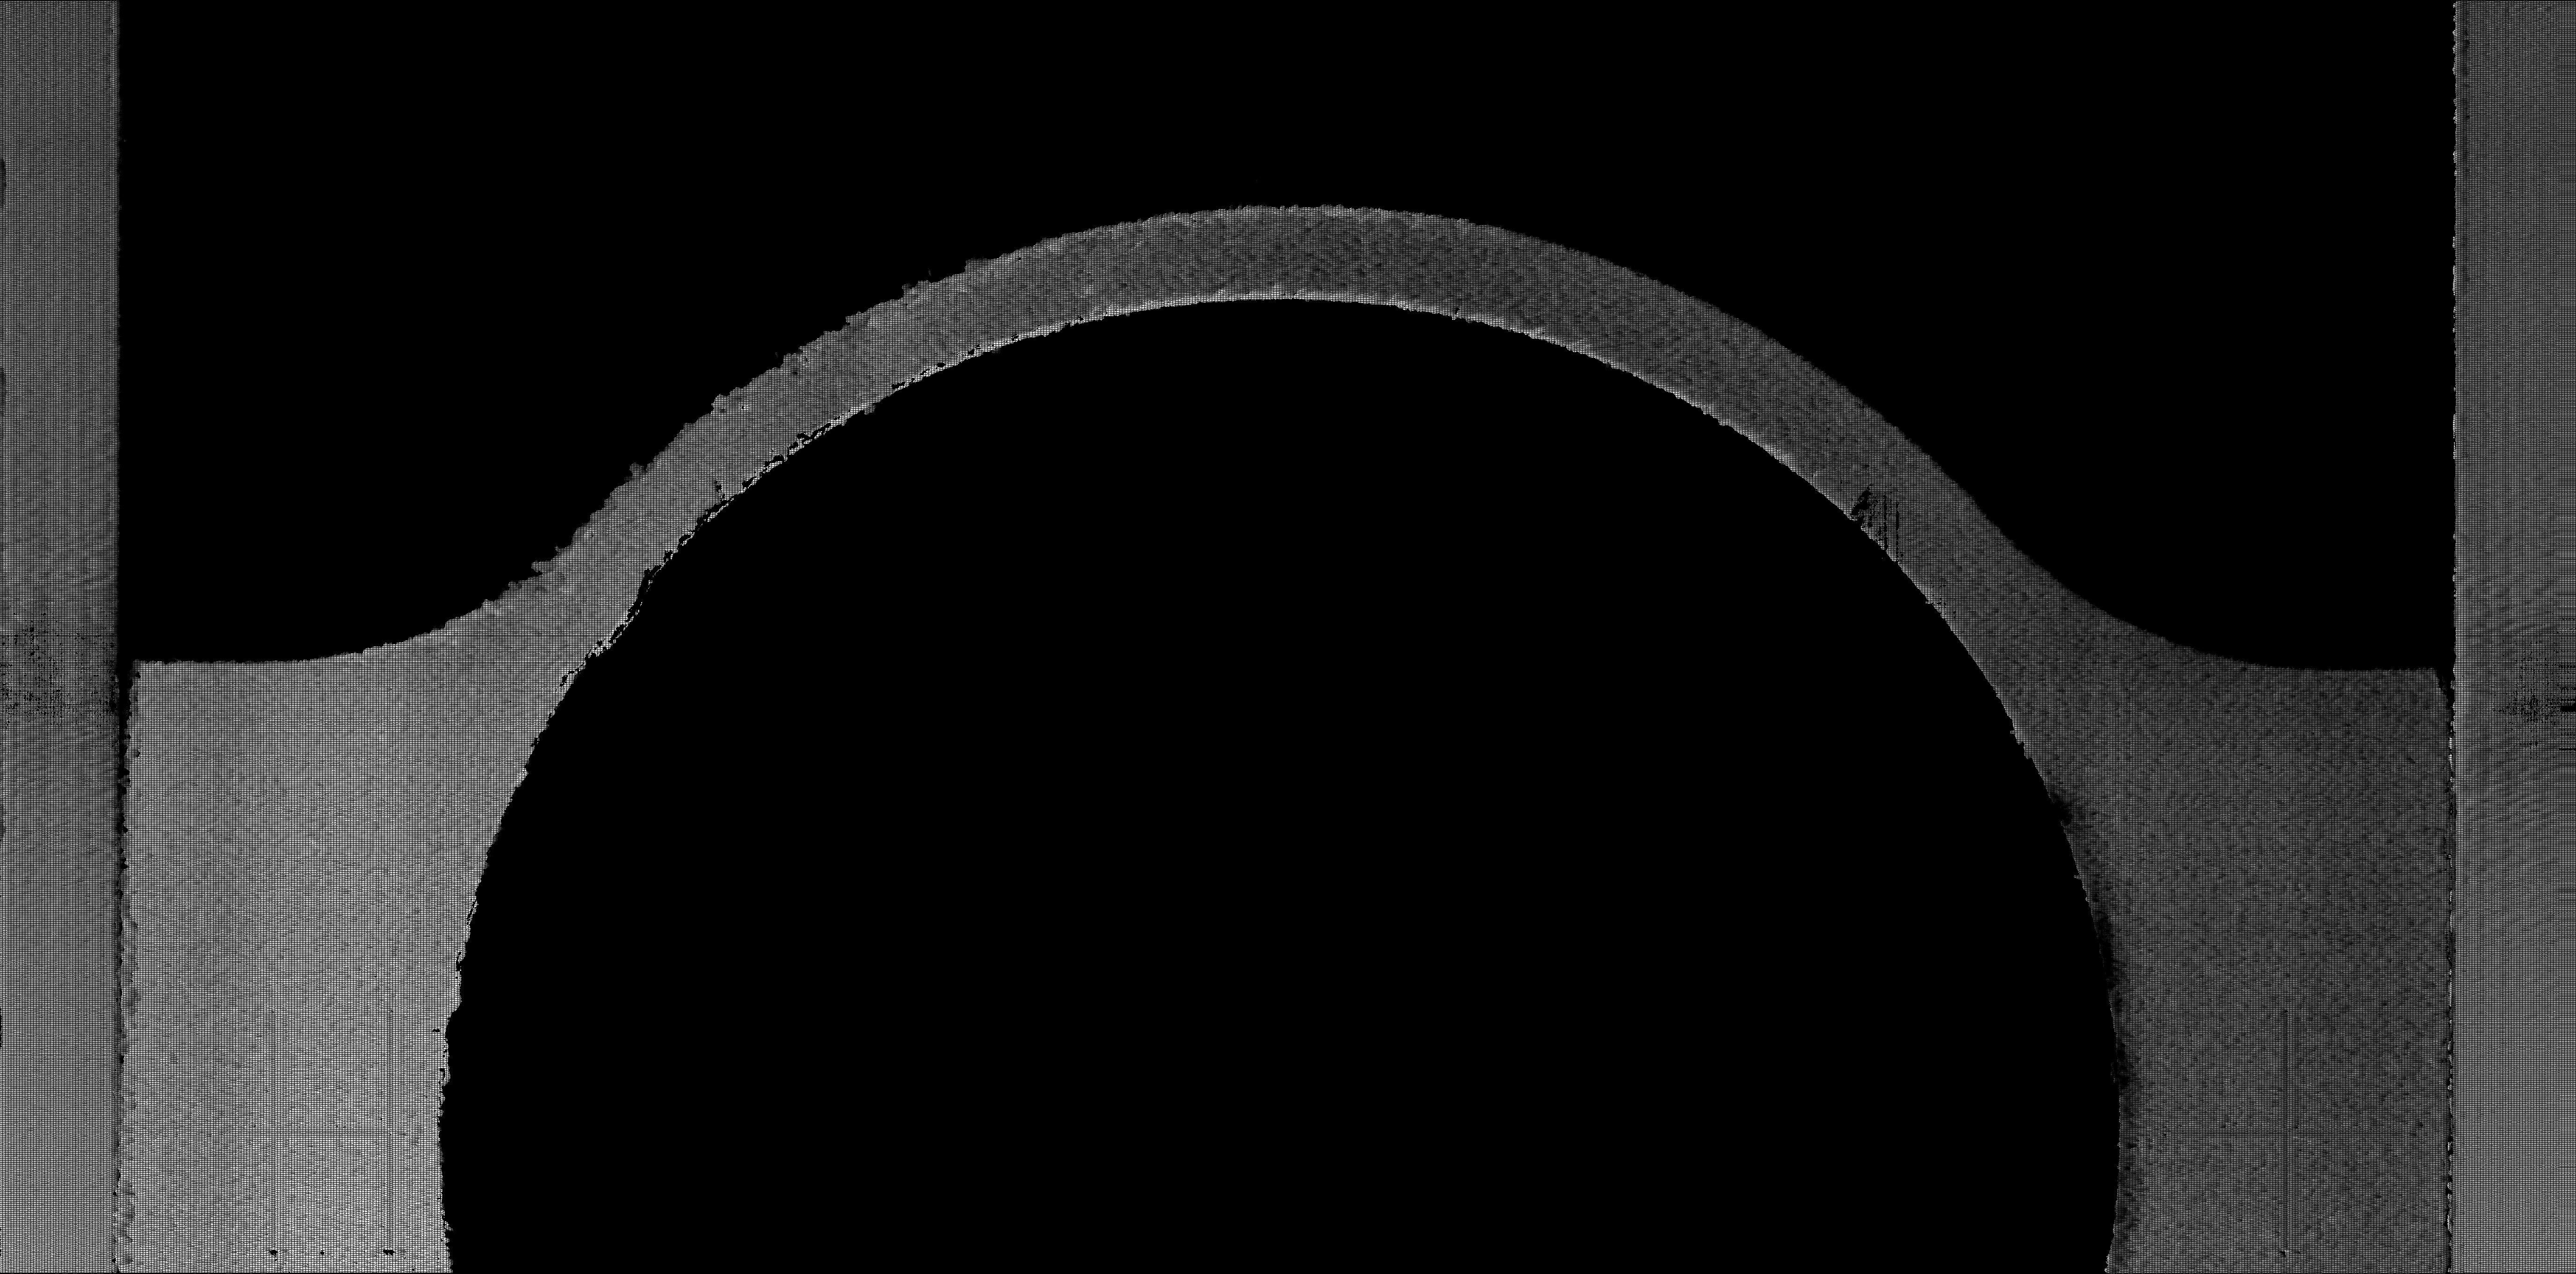
\includegraphics[width=0.4\textwidth]{images/am_sp0_top_10p.png}
    \caption{Metallteil gefiltert}\label{fig:metall_image}
\end{wrapfigure}

Man sieht vor allem auf der rechten Seite, dass Ränder nicht mehr klar erkennbar sind, 
da sie durch die Filterung Lücken aufweisen. Praxistest haben gezeigt das ein 
ausreichend gut funktionierender Filterwert 50 Prozent ist. Damit werden genug 
Messfehler aus dem Bild genommen aber trotzdem bleiben Oberflächenfeatures und Ränder
sichtbar genug um ein korrektes Zusammenfügen zu gewährleisten.
Dieses Filtern bezieht sich aber nur auf 2 dimensionale Bildinformationen.
Um bei dem Konvertieren noch weniger Punkte die nicht auf dem Bauteil liegen nicht in das Bild zu übernehmen, kann auch noch die Pointcloud gefiltert werden.
Hier kann ein einzelner Punkt relativ zu seinem Nachbarn im 3 dimensionalen Raum betrachtet werden, 
um so Ausreißer zu erkennen. Dafür sind in der Open-Source
Bibliothek 'Open3D' 2 Methoden vorhanden: Radius basiert oder auf Basis von 
statistischen Werten, erste Methode eignet sich gut, wenn die Maße des Objekts bekannt
sind. Hier wird um jeden Punkt eine Kugel gebildet und die Punkte die weniger als 
einen konfigurierbare Menge an Punkte in ihrer Kugel haben werden entfernt. Da 
das hier zu entwickelnde Verfahren sich nicht auf eine Bauteilgeometrie beschränken
ist dieses Verfahren nicht geeignet. Stattdessen wird das andere benutzt. Hier werden
die Punkte entfernt die weiter von ihren benachbarten Punkten entfernt sind als der 
durchschnittliche Abstand der Punkte in der gesamten Pointcloud. Hier kann die Menge der 
benachbarten Punkte die betrachtet werden sollen und ein Limit für den Abstand von der 
Standardabweichung. Umso mehr benachbarte Punkte betrachtet werden, umso mehr Zeit 
braucht die Filterung, aber die Filterung wird auch akkurater. Im Praxistest haben sich
hier 50 Nachbarpunkte bewährt. Mit diesem Wert werden bei Pointclouds in unserem 
Datensatz jeweils ca. 2 Prozent der Punkte entfernt. So kann das resultierende
Bild gut genug umgewandelt werden, um eine erfolgreiche Zusammenführung 
von verschiedenen Bildern zu gewährleisten.
Ein Nachteil bei der Filterung in Abbildung \ref{fig:image_from_pc} links und rechts 
mittig zu sehen. Hier sind schwarze Punkte sichtbar. Diese treten auf, weil der Scanner
hier über dem Bauteil Punkte erkannt hat. Durch das Filtern wurden diese Punkte entfernt
beziehungsweise bei der Konvertierung nicht berücksichtigt. Da diese Punkte dann fehlen
bleiben sie im resultierenden Bild schwarz. Das ist zwar etwas unschön anzuschauen, 
beeinträchtigt das zusammenfügen aber nicht weiter. 

\end{document}

%\newpage

\input{sections/6_Datenaufbereitung.tex}

\newpage

\documentclass[../main.tex]{subfiles}
\begin{document}

\section{Stitching}


\end{document}

\newpage

\documentclass[../main.tex]{subfiles}
\begin{document}

\section{Analyse der spannkraftinduzierten Deformation}

\subsection{Aufgenomme Daten auswerten}

\subsection{Deformationen erkennen}

\end{document}

\newpage


\chapter{Anwendung und Algorithmus}

Ziel dieser Arbeit ist es nicht nur eine Methodik zur optische 
Deformationserkennung zu entwickeln, sondern diese Methodik auch in einer 
Anwendung einfach nutzbar zu machen. 

Diese Kapitel dokumentiert diese Anwendung und geht auf Herausforderungen 
in der Entwicklung ein.

\section{Anwendung}

Die Anwendung beinhaltet verschiedene Funktionen, alle Funktionen 
können separat benutzt werden. Dadurch müssen zeitintensive Vorgänge nicht 
wiederholt werden, sondern Zwischenergebnisse können abgespeichert und 
neu geladen werden.
Die Anwendung bietet Funktionen, um Resultate in dem entsprechenden Dateiformat zu 
speichern. Soweit möglich werden Dateinamen Empfehlungen automatisch ermittelt, 
daher ist es zu empfehlen von Anfang an mit einem einheitlichen Namensschema bei
den 3D-Scannerdaten zu arbeiten. 
Das Schema \glqq Bauteilbeschreibung \textunderscore Spannungsstufe\grqq~~
\textunderscore Scannerdurchlauf.ply
wird empfohlen. Ein Beispiel für die zweite Pointcloud eines FDM-Bauteil bei der
vierten Spannungsstufen wäre also \glqq FDM0\textunderscore SP4\textunderscore 2.ply\grqq~.
In Abbildung \ref{fig:software_screenshot} ist die Oberfläche der Anwendung zu sehen.

\begin{figure}[H]
    \centering
    \includegraphics[width=0.9\textwidth]{images/software_screenshot.png}
    \caption{Anwendungsoberfläche}
    \label{fig:software_screenshot}
\end{figure}

Über die Buttons \glqq Select Pointcloud\grqq~ können Pointclouds zum Konvertieren in Bilder
ausgewählt werden. Der Text neben dem Bild zeigt den Dateinamen der ausgewählten 
Datei an. Die obere Pointcloud sollte hier als erstes ausgewählt werden.
Der Button \glqq Start PC conversion\grqq~~startet die Konvertierung. Der Balken 
daneben zeigt den Prozessfortschritt. 
Wenn \glqq Show Pointclouds\grqq~ gesetzt ist, werden die Pointclouds vor dem 
Konvertieren in einem separaten Fenster angezeigt. So kann überprüft werden, ob die 
korrekte Pointcloud ausgewählt wurde.
Wenn der Prozess abgeschlossen ist, werden die resultieren Bilder als Vorschau in der 
Anwendung angezeigt und die Option zum Speichern der Bilder ist nicht mehr ausgegraut.
Zusätzlich wird nach dem Konvertierungsprozess die Schaltfläche 
\glqq Stitch converted\grqq~ freigeschaltet. Durch diese Option können die 
Bilder direkt zusammengefügt werden, ohne das die Bilder extra gespeichert und 
eingeladen werden müssen. Wenn schon existierende Bilder zusammengefügt werden sollen, 
können die Schaltflächen \glqq Select top image\grqq und \glqq Select bot image\grqq
ausgewählt werden um das obere und untere Bild auszuwählen. Auch hier wird die 
ausgewählte Datei als Text angezeigt. Die Dateiauswahl erfolgt über das 
Windows-Kontextmenü, der zuletzt verwendete Ordner wird hierbei erhalten, sodass das 
zweite Bild schneller ausgewählt werden kann. 
Über den Button \glqq Start stitching\grqq wird der stitching Prozess gestartet. 
Auch hier wird der Fortschritt und das Endresultat, sobald es vorliegt, angezeigt.

Damit auch die CAD-Datei des additiv gefertigten Bauteils verglichen werden kann, 
existiert der \glqq Convert stl\grqq~ Button. Hier wird eine .stl Datei zu einem Bild 
konvertiert und kann über \glqq save stl\grqq~ gespeichert werden.

Mithilfe der rechts zu sehenden Schaltflächen können Bilder auf ihre Deformation hin 
verglichen werden. Die resultieren Deformationsdaten werden automatisch als Textdatei
in dem Ordner \glqq deformation\underline data\grqq~ gespeichert. Dieser Ordner wird automatisch 
in dem Verzeichnis erzeugt, in dem die Anwendung ausgeführt wird. 
Die erstellten Textdateien können mithilfe des Buttons \glqq Plot data\grqq~ ausgewählt 
werden, und werden automatisch als Graph angezeigt. 

Beim Konvertieren und stitchen werden alle Prozesse, die nicht voneinander abhängig sind,  
nebenläufig ausgeführt. Das reduziert die Laufzeit der Prozesse.

Die Anwendung ist in Python geschrieben, rechenintensive Prozesse wurden aber mithilfe 
der Bibliothek \glqq Numba\grqq~in optimierten Maschinencode compiliert~\cite{numba}.
Dadurch ist der Konvertierungs- und Stitching-Prozess deutlich schneller geworden. 
Durch die Optimierungen konnte der Konvertierungsprozess von 49 s auf 41 s verschnellert 
werden. Bei dem Stitchprozess war die Verbesserung noch deutlicher. Hier 
beträgt die Laufzeit mit Optimierungen ca. 30 s um zwei Konturen zu vergleichen. 
Ohne Optimierungen braucht der Vergleich derselben beiden Konturen 
hochgerechnet 600 Minuten.





\newpage


\chapter{Zusammenfassung und Ausblick}

[Stichpunkte]

\begin{itemize}
    \item Auf die Unterschiede der Materialen eingehen. Auch auf die ähnlichkeiten 
    wo die Deformation auftreten.
    \item Was das für die Bauteile bedeutet.
    \item Verbesserung: Stitching verbessern um einheitlichere Ergebnisse zu erhalten.
    \item Forschungsansätze: Veränderung in der inneren Struktur der Bauteile 
    vergleichen.
\end{itemize}


\newpage


\chapter{Validierung}

Im folgenden Kapitel wird die Deformationerkennung analysiert und überprüft.
Zur Überprüfung werden Materialeigenschaften und aufgenommene Messwerte 
mit der erkannten Deformation verglichen.

\section{Messergebnisse}

Es wurden fünf Bauteile mit verschiedenen Spannungsstufen gemessen. Für jede 
Spannungsstufe wurde die Kraft, die auf das Bauteil wirkte sowie die Verschiebung 
des Schraubstocks gemessen.
Jede Spannungsstufe wurde durch Stufenweises anziehen des Schraubstocks erreicht.
Die Spannkraftkurve eines einzelnen Einspannvorgangs ist in 
Abbildung \ref{fig:single} zu sehen. 
In der Spannungskurve ist ein elastischer Bereich für das 
Bauteil zu sehen, in dem sich die Spannkraft zurückbewegt, nachdem kein 
Anzugdrehmoment mehr anliegt. Aus diesem Grund kann nicht der maximale Wert der Spannkraft angenommen werden, 
sondern es muss ein Wert gewählt werden der nach dem maximalen Ausschlag liegt.
Dieser wurde über die erste Ableitung der Spannkraftkurve gefunden. Sobald der 
Absolutwert der Steigung unter 0.0009 N fällt, wir die Spannkraft und Auslenkung an 
diesem Punkt gewählt. 0.0009 N wurde empirisch ermittelt, um bei allen Bauteilen einen 
angemessenen Wert zu liefern.
Die Spannkraft wurde an zwei Achsen aufgenommen und zu der Gesamtkraft aufsummiert.

\begin{figure}[H]
    \centering
    \includegraphics[width=0.99\textwidth]{images/spannkraftstufen_single.png}
    \caption{Kraft- und Verschiebung der Spannungsstufe fünf bei einem FDM Bauteil}
    \label{fig:single}
\end{figure}

Diese maximalen Werte für die Spannkraft und Auslenkung wurden für jedes Bauteil 
akkumuliert und sind in Abbildung \ref{fig:akkumulated} dargestellt. 
Die mit dem FDM-Prozess hergestellten Bauteile wurden jeweils in sechs Spannungsstufen
gemessen. Zwischen den Stufen wurde versucht, eine konstante Kraft auf das Bauteil 
auszuüben. Durch den manuellen Prozess des Anziehens des Schraubstocks war dies 
jedoch nicht immer möglich.
Die Metallbauteile unterscheiden sich durch ihren Aufbau. 
Alle basieren auf dem gleichen 3D-Modell, besitzen jedoch unterschiedliche 
Stützstrukturen. Im Bauteil AM0 ist die vollständige Stützstruktur vorhanden,
während in den Bauteilen AM1 und AM2 die Stützstruktur in unterschiedlicher 
Tiefe ausgebohrt wurde. Die Bauteile sind in Abbildung \ref{fig:am_parts} dargestellt.

Das Bauteil AM0 wurde nur mit zwei Spannungsstufen gemessen, 
da bereits bei der zweiten Stufe über 2500 N Kraft erforderlich war, 
um das Bauteil nur minimal in x-Richtung zu deformieren. Dies zeigt, 
dass die Stützstruktur einen erheblichen Einfluss auf die Verformbarkeit 
eines Bauteils hat. Beim Bauteil AM1 wurden 2500 N erst nach vier Spannungsstufen 
erreicht. Vergleicht man die Verformung in x-Richtung mit der Verformung von AM2,
 zeigt sich, dass das Bauteil ohne Stützstruktur bei ähnlicher Krafteinwirkung 
 etwa doppelt so weit in x-Richtung deformiert wurde.

 Die FDM-Bauteile wurden mit deutlich weniger Kraft eingespannt. 
 Hier wurde bei etwa 250 N gestoppt, dennoch ist die Verschiebung der 
 Teile deutlich größer als bei den AM-Bauteilen. Diese Werte wurden aufgenommen, 
 um die visuelle Deformationserkennung zu validieren.

\begin{figure}[H]
    \centering
    \includegraphics[width=0.99\textwidth]{images/spannkraftstufen_akkumuliert.png}
    \caption{Akkumulierte Kraft und Verschiebung, mit der jedes Bauteil deformiert wurde.}
    \label{fig:akkumulated}
\end{figure}

\begin{figure}[H]
    \centering
    \begin{minipage}{.33\textwidth}
      \centering
      \includegraphics[width=0.9\linewidth]{images/AM0_crop.JPG}
      \caption*{(a)}
    \end{minipage}%
    \begin{minipage}{.33\textwidth}
      \centering
      \includegraphics[width=0.9\linewidth]{images/AM1_crop.JPG}
      \caption*{(b)}
    \end{minipage}
    \begin{minipage}{.33\textwidth}
        \centering
        \includegraphics[width=0.9\linewidth]{images/AM2_crop.JPG}
        \caption*{(c)}
      \end{minipage}
      \caption{(a): AF Metallbauteil mit voller Stützstruktur, Bezeichnung: AM0.
      (b): AF Bauteil mit der halben Stützstruktur ausgebohrt, Bezeichnung: AM1.
      (c): AF Bauteil ohne Stützstruktur, Bezeichnung: AM2}
      \label{fig:am_parts}
\end{figure}

\section{Ergebnisse der optischen Deformationsanalyse}

In Abbildung \ref{fig:am_defos} und Abbildung \ref{fig:fdm_defos} sind die erkannten,
vertikalen Deformation grafisch dargestellt. Jeweils von Spannungsstufe null bis 
Spannungsstufen Sechs. Bei dem FDM Bauteil fehlt die Spannungsstufen fünf, 
diese ist leider bei der händischen Dateiname Vergabe überschrieben worden und konnte 
deshalb nicht ausgewertet worden. Aus diesem Grund ist eine so große Lücke in der 
Abbildung \ref{fig:fdm_defos}.
Außerdem sind große Unterschiede in der absoluten Deformation zu sehen. Zum Beispiel 
die rote Kurve in Abbildung \ref{fig:am_defos} die den Unterschied der Spannungsstufen 
null und eins angibt. Diese Kurve sollte näher an null der y-Achse liegen. 
Dies liegt an Ungenauigkeiten in dem Stitching Verfahren. In den Graphen ist also 
auf die Steigung der Deformationskurve zu achten. In der Steigung erkannt man das 
sich die Bauteile in mittleren Bereich nach außen hin deformiert haben und in 
den Randbereichen sich nach innen und dann wieder nach außen deformieren.
Außerdem ist im Vergleich der beiden Graphen zu sehen das sich das FDM Bauteil deutlich 
mehr verformt hat. Hier beträgt die größte Deformation über 150 Pixel.
Bei dem Metallbauteil, das mit der zehnfachen Kraft eingespannt wurde (250 nm vs. 2500 nm)
sind es nur knapp 40 Pixel, wie in Abbildung~\ref{fig:deformation_data_am} zu sehen. Trotzdem ist zu sehen das sich die Bauteile, die auch die 
gleiche Geometrie teilen, auf die gleiche Weise verformt haben.

\begin{figure}[H]
  \centering
  \includegraphics[width=0.95\textwidth]{images/am2_all_defos.png}
  \caption{Sechs Deformationsstufen bei einem additiv gefertigten Metallbauteil ohne
  Stützstruktur von 0 bis 2500 nm}
  \label{fig:am_defos}
\end{figure}

\begin{figure}[H]
  \centering
  \includegraphics[width=0.95\textwidth]{images/fdm2_all_defos.png}
  \caption{Fünf Deformationsstufen bei einem FDM Bauteil von 0 bis 250 nm}
  \label{fig:fdm_defos}
\end{figure}

\begin{figure}[H]
    \centering
    \includegraphics[width=0.9\textwidth]{images/AM_sp0_sp2_defo_plot.png}
    \caption{Differenz von zwei Spannungsstufen bei einem additiv gefertigten Metallbauteil, 
    das zur Hälfte mit Stützstrukturen gefüllt ist (Abbildung~\ref{fig:am_parts (b)}). }
    \label{fig:deformation_data_am}
\end{figure}

\section{Beurteilung der Ergebnisse}

Grundsätzlich ermöglicht die Methode die Erkennung und den Vergleich von Deformationen 
eines Bauteils. Die gemessene Deformation eines Bauteils entspricht den erwarteten Werten, 
abhängig von Material und Geometrie des Bauteils. FDM-gedruckte Kunststoffteile zeigen 
eine deutlich stärkere Verformung im Vergleich zu Metallteilen.
Bei den Metallteilen zeigt sich, dass das Vorhandensein einer Stützstruktur die
Verformung des Bauteils signifikant reduziert. 
Die unterschiedlichen Deformationen sind in Abbildung \ref{fig:materials} dargestellt. 
Das in Abbildung \ref{fig:am_parts} (a) gezeigte Bauteil konnte nicht analysiert werden, 
da durch die Stützstruktur keine korrekte Transformation zur stitchen berechnet werden konnte.
Bei den FDM-Bauteilen ist festzustellen, dass sie sich deutlich stärker verformen 
als die Metallteile. Beide FDM-Bauteile zeigen eine ähnliche Verformungsausprägung, 
jedoch tritt die Deformation, trotz identischer Geometrie, an unterschiedlichen Stellen auf. 
Dies könnte auf Unterschiede im Druckprozess zurückzuführen sein. 
Diese Beobachtung zeigt einen weiteren Nutzen der Methodik: Sie ermöglicht
nicht nur die Bestimmung des Ausmaßes der Deformation, sondern auch die 
Identifikation von Schwachstellen innerhalb eines Bauteils, die zu einer erhöhten 
 
Deformation führen.

\begin{figure}[H]
  \centering
  \includegraphics[width=0.95\textwidth]{images/compare_materials.png}
  \caption{Vergleich von Materialien und Bauteilgeometrien}
  \label{fig:materials}
\end{figure}

Dennoch ist die Deformationserkennung noch nicht perfekt. 
Fehler im Stitching Prozess führen zu starken Änderungen in der Deformationserkennung. 
Wie in Abbildung \ref{fig:errors} zu sehen ist, kann sich die Breite des Bauteils 
zwischen zwei Spannungsstufen unterscheiden. Er ist erkennbar, dass der Rand der einen 
Kontur, repräsentiert durch die magenta gefärbte Linie, immer größer ist als 
der Rand der anderen Kontur, hier in blau dargestellt.
Dieser Versatz entsteht, weil beim Stitching eine Transformation verwendet wurde die sich 
um wenige Pixel unterscheidet. Dadurch wächst auch die erkannte Deformationen.
Aus diesem Grund existieren in den Abbildungen \ref{fig:am_defos} und \ref{fig:fdm_defos}
Linien die nicht dem erwarteten Verhalten entsprechen. 
In Abbildung \ref{fig:fdm_defos} zum Beispiel, sollte die Deformation zwischen den 
Spannungsstufen eins und zwei 
(in rot dargestellt) am kleinsten sein. Stattdessen liegt die Kurve bei -50 Pixeln im Graph.

\begin{figure}[H]
  \centering
  \includegraphics[width=0.95\textwidth]{images/contours_matching_36.png}
  \caption{Vergleich von Konturen aus nicht korrekt zusammengefügten Bildern.}
  \label{fig:errors}
\end{figure}

Zusätzlich kann, bei Bildern ohne klare Konturen, das Stitching nicht korrekt durchgeführt
werden. Dies ist bei den additiv gefertigten Metallbauteil mit Stützstruktur der Fall 
(Abbildung \ref{fig:am_parts} (a)). Das Bild, das aus dem Scan dieses Bauteils erstellt wurde, 
ist in Abbildung \ref{fig:errorimage} zu sehen. Es lassen sich keine eindeutigen Konturen 
erkennen, die für das Stitching genutzt werden könnten.

\begin{figure}[H]
  \centering
  \includegraphics[width=0.95\textwidth]{images/am0.png}
  \caption{Bild eines Scans von einem Metallbauteil mit Stützstruktur.}
  \label{fig:errorimage}
\end{figure}




\newpage
\bibliography{quellen}
\bibliographystyle{alpha}

\end{document}